\documentclass[11pt,a4paper]{article}
\usepackage{gtu-el-yazisi}
\begin{document}
\notbilgi{İşaretler ve Sistemler}{Ders 13 -- z-Transformu}{Isaret-ve-Sistemler-ders-13.pdf}
\providecommand{\yalti}[1]{{\color{yesilkalem}\underline{\color{murekkep}#1}}}

\section{z-transformu}
\sayfa{1}
\begin{align*}
  &X(z)=\sum_{n=-\infty}^{\infty}x[n]z^{-n}\\
  &x[n]\ \overset{\mathcal{Z}}{\longleftrightarrow}\ X(z)\\
  &X(z)=\mathcal{Z}\{x[n]\}
\end{align*}
\[
  \Rightarrow z=re^{j\omega}\ \
  \begin{array}{l}
    \longrightarrow r:\ \text{magnitude}\\
    \hookrightarrow \omega:\ \text{angle}
  \end{array}
\]
\[
  X(z)=X(re^{j\omega})=\sum_{n=-\infty}^{\infty}x[n](re^{j\omega})^{-n}=\sum_{n=-\infty}^{\infty}x[n]r^{-n}e^{-j\omega n}=\mathcal{F}\{x[n]r^{-n}\}
\]
$\Rightarrow z=e^{j\omega}$ \ $(r=1)$
\[
  X(z)=X(e^{j\omega})=\sum_{n=-\infty}^{\infty}x[n]e^{-j\omega n}=\mathcal{F}\{x[n]\}=X(z)\Big|_{z=e^{j\omega}}
\]
\begin{center}
  \begin{tikzpicture}[scale=0.9]
    \draw[->] (-2,0) -- (2.2,0) node[right] {Re};
    \draw[->] (0,-1.6) -- (0,1.8) node[above] {Im};
    \draw[murekkep, thick] (0,0) circle (1.2);
    \draw[dashed] (0,0) -- (60:1.9) node[above right] {$z=e^{j\omega}$};
    \draw (0.35,0) arc (0:60:0.35); \node at (25:0.6) {\scriptsize$\omega$};
    \node[below right] at (1.2,0) {\scriptsize$1$};
    \node[right] at (-30:1.3) {Birim çember};
    \node at (0,-2) {$z$-düzlemi};
  \end{tikzpicture}
\end{center}
$\Rightarrow$ \textbf{Yakınsama bölgesi (region of convergence):} z-transform toplamının yakınsadığı $z$ değer aralığıdır.

\textbf{Not:} z-transformunun ROC'u birim çemberi içerirse Fourier transformu yakınsar.

\begin{ornek}[]
  $x[n]=a^nu[n]$
\end{ornek}
\[
  X(z)=\sum_{n=-\infty}^{\infty}x[n]z^{-n}=\sum_{n=-\infty}^{\infty}a^nu[n]z^{-n}=\sum_{n=0}^{\infty}\bigl(az^{-1}\bigr)^n
\]
Reminder: \quad $\displaystyle\sum_{k=0}^{\infty}\alpha^k=\frac{1}{1-\alpha},\ \ |\alpha|<1$
\[
  X(z)=\frac{1}{1-az^{-1}}=\frac{z}{z-a},\ \ |az^{-1}|<1,\ \ |z|>|a|
\]

\sayfa{2}
\[
  \left.
  \begin{array}{l}
    a^nu[n]\ \overset{\mathcal{Z}}{\longleftrightarrow}\ \dfrac{1}{1-az^{-1}},\ \ |z|>|a|\\[4mm]
    u[n]\ \longleftrightarrow\ \dfrac{1}{1-z^{-1}},\ \ |z|>1
  \end{array}
  \ \right)\ a=1
\]
\noindent
\begin{minipage}[c]{0.55\linewidth}
  \centering
  \begin{tikzpicture}[scale=0.9]
    \foreach \a in {0,20,...,340} \draw[kursunkalem] (\a:0.75) -- (\a:1.75);
    \draw[->] (-2,0) -- (2.2,0) node[right] {Re};
    \draw[->] (0,-1.9) -- (0,2) node[above] {Im};
    \draw[murekkep, thick] (0,0) circle (1.3);
    \draw[dashed, thick] (0,0) circle (0.75);
    \draw[thick] (0,0) circle (0.08);
    \node at (0.75,0) {$\times$};
    \node[above right] at (0.7,0) {\scriptsize$a$};
    \node[below right] at (1.3,0) {\scriptsize$1$};
    \node at (0,-2.3) {$z$-düzlemi / kutup-sıfır çizimi};
  \end{tikzpicture}
\end{minipage}\hfill
\begin{minipage}[c]{0.4\linewidth}
  $\times$: kutup\\[1mm]
  $\circ$: sıfır\\[3mm]
  $0<a<1$
\end{minipage}

\begin{ornek}[]
  $x[n]=-a^nu[-n-1]$
\end{ornek}
\begin{align*}
  X(z)&=\sum_{n=-\infty}^{\infty}x[n]z^{-n}=-\sum_{n=-\infty}^{\infty}a^nu[-n-1]z^{-n}=-\sum_{n=-\infty}^{-1}a^nz^{-n}=-\sum_{n=1}^{\infty}a^{-n}z^{n}=1-\sum_{n=0}^{\infty}\bigl(a^{-1}z\bigr)^n\\
  &=1-\frac{1}{1-a^{-1}z}=\frac{1}{1-az^{-1}}=\frac{z}{z-a},\ \ |a^{-1}z|<1,\ \ |z|<|a|
\end{align*}
\[
  -a^nu[-n-1]\ \overset{\mathcal{Z}}{\longleftrightarrow}\ \frac{1}{1-az^{-1}},\ \ |z|<|a|
\]
\begin{center}
  \begin{tikzpicture}[scale=0.9]
    \begin{scope}
      \clip (0,0) circle (0.75);
      \foreach \i in {-2,-1.8,...,1} \draw[kursunkalem] (\i,-1) -- ++(1,2);
    \end{scope}
    \draw[dashed] (0,0) circle (0.75);
    \draw[->] (-2,0) -- (2.2,0) node[right] {Re};
    \draw[->] (0,-1.9) -- (0,2) node[above] {Im};
    \draw[murekkep, thick] (0,0) circle (1.4);
    \draw[thick] (0,0) circle (0.08);
    \node at (0.75,0) {$\times$};
    \node[below right] at (0.7,0) {\scriptsize$a$};
    \node[above right] at (1.4,0) {\scriptsize$1$};
  \end{tikzpicture}
  \qquad $0<a<1$
\end{center}
$X(z)$'in ROC'u birim çemberi içermediğinden, $x[n]$'nin Fourier Transformu yoktur.

\begin{ornek}[]
  $x[n]=7\bigl(\frac13\bigr)^nu[n]-6\bigl(\frac12\bigr)^nu[n]$
\end{ornek}
Reminder: \quad $a^nu[n]\ \overset{\mathcal{Z}}{\longleftrightarrow}\ \dfrac{1}{1-az^{-1}},\ \ |z|>|a|$
\[
  X(z)=\underbrace{\frac{7}{1-\frac13z^{-1}}}_{\substack{|\frac13z^{-1}|<1\\ |z|>1/3}}
  -\underbrace{\frac{6}{1-\frac12z^{-1}}}_{\substack{|\frac12z^{-1}|<1\\ |z|>1/2}}
  =\frac{1-\frac32z^{-1}}{\bigl(1-\frac13z^{-1}\bigr)\bigl(1-\frac12z^{-1}\bigr)}
  =\frac{z(z-3/2)}{(z-1/3)(z-1/2)},\ \ |z|>1/2
\]

\sayfa{3}
\begin{center}
  \begin{tikzpicture}[scale=1.4]
    \foreach \a in {0,18,...,342} \draw[kursunkalem] (\a:0.5) -- (\a:1.35);
    \draw[->] (-1.5,0) -- (1.9,0) node[right] {Re};
    \draw[->] (0,-1.4) -- (0,1.5) node[above] {Im};
    \draw[murekkep, thick] (0,0) circle (1);
    \draw[dashed, thick] (0,0) circle (0.5);
    \draw[thick] (0,0) circle (0.05);
    \draw[thick] (1.5,0) circle (0.05);
    \node at (0.333,0) {$\times$}; \node at (0.5,0) {$\times$};
    \node[below] at (0.3,-0.05) {\scriptsize$1/3$};
    \node[below right] at (0.48,-0.05) {\scriptsize$1/2$};
    \node[above right] at (1,0) {\scriptsize$1$};
    \node[below] at (1.5,-0.05) {\scriptsize$3/2$};
  \end{tikzpicture}
\end{center}

\begin{ornek}[]
  $x[n]=\bigl(\frac13\bigr)^n\sin\bigl(\frac{\pi n}{4}\bigr)u[n]$, \ $X(z)=\,?$
\end{ornek}
\[
  x[n]=\frac{1}{2j}\Bigl(\frac13e^{j\pi/4}\Bigr)^nu[n]-\frac{1}{2j}\Bigl(\frac13e^{-j\pi/4}\Bigr)^nu[n]
\]
\[
  X(z)=\underbrace{\frac{1}{2j}\,\frac{1}{1-\frac13e^{j\pi/4}z^{-1}}}_{|\frac13e^{\yalti{j\pi/4}}z^{-1}|>1}
  -\underbrace{\frac{1}{2j}\,\frac{1}{1-\frac13e^{-j\pi/4}z^{-1}}}_{|\frac13e^{-j\pi/4}z^{-1}|>1}
  =\frac{z/3\sqrt2}{\bigl(z-\frac13e^{j\pi/4}\bigr)\bigl(z-\frac13e^{-j\pi/4}\bigr)},\ \ |z|>1/3\text{\footnotemark}
\]
\footnotetext{Claude notu: geometrik serinin yakınsaması için koşullar muhtemelen $|\cdot|<1$ olmalı; bu da yazılan $|z|>1/3$ sonucunu verir.}

\textbf{Not:}
\[
  \text{Payın derecesi}\ \begin{array}{l} >\\ <\end{array}\ \text{paydanın derecesi}\ \
  \begin{array}{l}
    \longrightarrow \text{sonsuzda kutup vardır}\\
    \longrightarrow \text{sonsuzda sıfır vardır}
  \end{array}
\]

\subsection{Yakınsaklık bölgesi (ROC) özellikleri}
\begin{enumerate}[label=\arabic*)]
  \item $X(z)$'nin ROC'u $z$-düzleminde orijin merkezli bir halkadan oluşur.
    \[ X(z)=X(re^{j\omega})=\sum_{n=-\infty}^{\infty}x[n]r^{-n}e^{-j\omega n}=\mathcal{F}\{x[n]r^{-n}\} \]
    \[ \sum_{n=-\infty}^{\infty}|x[n]|r^{-n}<\infty \]
  \item ROC, herhangi bir kutup içermez.
  \item $x[n]$ sonlu süreli ise, ROC, $\overset{\text{olası}}{z=0}$ ve/veya $z=\infty$ değerleri dışında bütün $z$-düzlemidir.
\end{enumerate}

\begin{ornek}[]
  $x[n]=\delta[n]$
\end{ornek}
\[
  X(z)=\sum_{n=-\infty}^{\infty}x[n]z^{-n}=\sum_{n=-\infty}^{\infty}\delta[n]z^{-n}\underset{\substack{\uparrow\\ \delta[n]=1,\ n=0}}{=}1
\]
\[
  \delta[n]\ \overset{\mathcal{Z}}{\longleftrightarrow}\ 1,\ \ \forall z\ \ (\text{ROC, } z=0 \text{ ve } z=\infty \text{ içeren bütün } z\text{-düzlemidir})
\]

\sayfa{4}
\begin{ornek}[]
  $x[n]=\delta[n-1]$
\end{ornek}
\[
  X(z)=\sum_{n=-\infty}^{\infty}x[n]z^{-n}=\sum_{n=-\infty}^{\infty}\delta[n-1]z^{-n}\underset{\substack{\uparrow\\ \delta[n-1]=1,\ n=1}}{=}z^{-1}=\frac1z
\]
$z=0$'da bir kutup var.\\
ROC, $z=\infty$ içeren, $z=0$ dışında bütün $z$-düzlemidir.

\begin{ornek}[]
  $x[n]=\delta[n+1]$
\end{ornek}
\[
  X(z)=\sum_{n=-\infty}^{\infty}\delta[n+1]z^{-n}\underset{\substack{\uparrow\\ \delta[n+1]=1,\ n=-1}}{=}z
\]
$z=\infty$'da bir kutup vardır.\\
ROC, $z=0$ içeren, $z=\infty$ dışında bütün $z$-düzlemidir.

\begin{enumerate}[label=\arabic*), start=4]
  \item $x[n]$ sağ yanlı ve $|z|=r_0$ çemberi ROC'da ise, $|z|>r_0$ sağlayan sonlu bütün $z$ değerleri de ROC'da olur.
    \begin{center}
      \begin{tikzpicture}[scale=0.5]
        \draw[->] (-3.5,0) -- (5,0) node[right] {$n$};
        \node[above] at (-2.6,1.6) {$x[n]$};
        \foreach \k in {-3,-2,-1} \fill[murekkep] (\k,0) circle (3pt);
        \foreach \k/\h in {0/1.2,1/1.8,2/0.9,3/2.1,4/1.4} {\draw[murekkep, thick] (\k,0) -- (\k,\h); \fill[murekkep] (\k,\h) circle (3pt);}
        \node[below] at (0,0) {\scriptsize$N_1$};
        \node at (-3.8,0.3) {$\cdots$};
        \node at (4.8,0.9) {$\cdots$};
      \end{tikzpicture}\hspace{2cm}
      \begin{tikzpicture}[scale=0.8]
        \foreach \a in {0,24,...,336} \draw[kursunkalem] (\a:0.9) -- (\a:1.6);
        \draw[dashed, thick] (0,0) circle (0.9);
        \draw[->] (-1.8,0) -- (1.9,0) node[right] {Re};
        \draw[->] (0,-1.7) -- (0,1.8) node[above] {Im};
      \end{tikzpicture}
    \end{center}
    \[
      X(z)=\sum_{n=N_1}^{\infty}x[n]z^{-n}\ \
      \begin{array}{l}
        \longrightarrow N_1<0 \text{ iken } z\to\infty,\ X(z) \text{ sonsuz olur ve ROC, } z=\infty \text{ içermez.}\\[1mm]
        \hookrightarrow x[n]=0,\ n<0 \text{ için } N_1\geq0 \text{ olur ve ROC, } z=\infty \text{ içerir.}
      \end{array}
    \]
    $\rightarrow$ sağ yanlı $x[n]$'nin ROC'u içi bir çember ile sınırlanmış, sonsuza doğru genişleyen (sonsuzu içerebilir) bir bölgedir.
  \item $x[n]$ sol yanlı ve $|z|=r_0$ çemberi ROC'da ise, $0<|z|<r_0$ sağlayan bütün $z$ değerleri de ROC'da olur.
    \begin{center}
      \begin{tikzpicture}[scale=0.5]
        \draw[->] (-4.5,0) -- (4,0) node[right] {$n$};
        \foreach \k/\h in {-4/1.0,-3/2.1,-2/1.7,-1/1.2,0/1.6} {\draw[murekkep, thick] (\k,0) -- (\k,\h); \fill[murekkep] (\k,\h) circle (3pt);}
        \foreach \k in {1,2,3} \fill[murekkep] (\k,0) circle (3pt);
        \node[below] at (0,0) {\scriptsize$N_2$};
        \node at (-4.9,0.9) {$\cdots$};
        \node at (3.3,0.4) {$\cdots$};
      \end{tikzpicture}\hspace{2cm}
      \begin{tikzpicture}[scale=0.8]
        \begin{scope}
          \clip (0,0) circle (0.9);
          \foreach \i in {-2.4,-2.1,...,1.2} \draw[kursunkalem] (\i,-1) -- ++(1.2,2);
        \end{scope}
        \draw[dashed, thick] (0,0) circle (0.9);
        \draw[->] (-1.8,0) -- (1.9,0) node[right] {Re};
        \draw[->] (0,-1.7) -- (0,1.8) node[above] {Im};
      \end{tikzpicture}
    \end{center}
    \[
      X(z)=\sum_{n=-\infty}^{N_2}x[n]z^{-n}\ \
      \begin{array}{l}
        \longrightarrow N_2>0 \text{ iken } z\to0,\ X(z) \text{ sonsuza gider ve ROC, } z=0 \text{ içermez.}\\[1mm]
        \hookrightarrow x[n]=0,\ n>0 \text{ için } N_2\leq0 \text{ olur ve ROC, } z=0 \text{ içerir.}
      \end{array}
    \]
    $\rightarrow$ sol yanlı $x[n]$'nin ROC'u dışı bir çember ile sınırlanmış, orijine doğru genişleyen (orijini içerebilir) bir bölgedir.
  \sayfa{5}
  \item $x[n]$ iki yanlı ve $|z|=r_0$ çemberi ROC'da ise, ROC, $z$-düzleminde $|z|=r_0$ çemberini içeren bir halkadır.
    \begin{center}
      \begin{tikzpicture}[scale=0.8]
        \foreach \a in {0,15,...,345} \draw[kursunkalem] (\a:1.05) -- (\a:1.5);
        \draw[dashed] (0,0) circle (1.05); \draw[dashed] (0,0) circle (1.5);
        \draw[->] (-1.9,0) -- (2.1,0) node[right] {Re};
        \draw[->] (0,-1.8) -- (0,1.9) node[above] {Im};
      \end{tikzpicture}
    \end{center}
  \item $X(z)$ rasyonel ise, ROC, ya kutuplarla sınırlıdır ya da sonsuza genişler ve kutup içermez.\\
    $\rightarrow$ $x[n]$ sağ yönlü ise, ROC, en dıştaki kutubun dışındaki $z$-düzlemidir.\\
    $\rightarrow$ $x[n]$ sol yönlü ise, ROC, en içteki sıfırdan farklı kutubun içindeki $z$-düzlemidir.
\end{enumerate}

\begin{ornek}[]
  $x[n]=b^{|n|}$, \ $b>0$
\end{ornek}
\begin{align*}
  X(z)&=\sum_{n=-\infty}^{\infty}x[n]z^{-n}=\sum_{n=-\infty}^{\infty}b^{|n|}z^{-n}=\sum_{n=-\infty}^{-1}b^{-n}z^{-n}+\sum_{n=0}^{\infty}b^nz^{-n}\\
  \sum_{n=-\infty}^{-1}b^{-n}z^{-n}&=-1+\sum_{n=0}^{\infty}(bz)^n=-1+\frac{1}{1-bz}=\frac{bz}{1-bz},\ \ |bz|<1,\ \ |z|<1/b\\
  \sum_{n=0}^{\infty}b^nz^{-n}&=\frac{1}{1-bz^{-1}},\ \ |bz^{-1}|<1,\ \ |z|>b
\end{align*}
\[ x[n]=b^{|n|}=b^{-n}u[-n-1]+b^nu[n] \]
\begin{align*}
  \text{Reminder:}\quad b^nu[n]\ &\overset{\mathcal{Z}}{\longleftrightarrow}\ \frac{1}{1-bz^{-1}},\ \ |z|>b\\
  b^{-n}u[n-1]\text{\footnotemark}\ &\overset{\mathcal{Z}}{\longleftrightarrow}\ \frac{-1}{1-b^{-1}z^{-1}},\ \ |z|<1/b
\end{align*}
\footnotetext{Claude notu: muhtemelen $b^{-n}u[-n-1]$ olmalı (bir üst satırdaki ayrışımla uyumlu).}
\[
  X(z)=\frac{1}{1-bz^{-1}}-\frac{1}{1-b^{-1}z^{-1}}=\frac{b^2-1}{b}\cdot\frac{z}{(z-b)(z-b^{-1})},\qquad b<|z|<1/b
\]
\begin{center}
  \begin{tikzpicture}[scale=0.5]
    \draw[->] (-5.6,0) -- (5.8,0) node[right] {$n$};
    \draw[->] (0,-0.2) -- (0,3.4) node[above right] {$x[n]$, \ $0<b<1$};
    \foreach \k in {-4,...,4} {
      \pgfmathsetmacro{\h}{2.6*0.78^(abs(\k))}
      \draw[murekkep, thick] (\k,0) -- (\k,\h); \fill[murekkep] (\k,\h) circle (3pt);}
    \node[right] at (0,2.75) {\scriptsize$1$};
    \node at (-5.3,0.6) {$\cdots$};
    \node at (5.1,0.6) {$\cdots$};
  \end{tikzpicture}\hspace{1.5cm}
  \begin{tikzpicture}[scale=0.9]
    \foreach \a in {0,12,...,348} \draw[kursunkalem] (\a:0.6) -- (\a:1.65);
    \draw[dashed] (0,0) circle (0.6); \draw[dashed] (0,0) circle (1.65);
    \draw[murekkep, thick] (0,0) circle (1.05);
    \draw[->] (-2,0) -- (2.4,0) node[right] {Re};
    \draw[->] (0,-1.9) -- (0,2) node[above] {Im};
    \draw[thick] (0,0) circle (0.07);
    \node at (0.6,0) {$\times$}; \node at (1.65,0) {$\times$};
    \node[below] at (0.6,-0.05) {\scriptsize$b$};
    \node[above left] at (1.05,0) {\scriptsize$1$};
    \node[above right] at (1.65,0) {\scriptsize$1/b$};
  \end{tikzpicture}
\end{center}

\section{Ters z-transform}
\sayfa{6}
\begin{align*}
  X(z)&=X(re^{j\omega})=\sum_{n=-\infty}^{\infty}x[n]r^{-n}e^{-j\omega n}=\mathcal{F}\{x[n]r^{-n}\}\\
  x[n]r^{-n}&=\mathcal{F}^{-1}\{X(re^{j\omega})\}=\frac{1}{2\pi}\int_{2\pi}X(re^{j\omega})e^{j\omega n}\,d\omega\\
  x[n]&=\frac{1}{2\pi}\int_{2\pi}X(re^{j\omega})(re^{j\omega})^n\,d\omega
\end{align*}
\[ z=re^{j\omega}\ \longrightarrow\ dz=jre^{j\omega}\,d\omega=jz\,d\omega \]
\[ x[n]=\frac{1}{2\pi j}\oint X(z)z^{n-1}\,dz \]
$\oint$: $r$ yarıçaplı, orijin merkezli, saat yönünün tersinde kapalı dairesel bir kontur etrafında alınan integrali gösterir.
\[
  X(z)=\sum_{i=1}^{m}\frac{A_i}{1-a_iz^{-1}}\ \
  \begin{array}{l}
    \longrightarrow x[n]=A_ia_i^nu[n]\ :\ \text{sağ yanlı}\\[1mm]
    \hookrightarrow x[n]=-A_ia_i^nu[-n-1]\ :\ \text{sol yanlı}
  \end{array}
\]

\begin{ornek}[]
  $X(z)=\dfrac{1}{\bigl(1-\frac13z^{-1}\bigr)\bigl(1-2z^{-1}\bigr)}=\dfrac{z^2}{\bigl(z-\frac13\bigr)(z-2)}=\dfrac{A}{1-\frac13z^{-1}}+\dfrac{B}{1-2z^{-1}}$,
  \qquad $A=-1/5$, \ $B=6/5$
\end{ornek}
\noindent
\begin{minipage}[t]{0.32\linewidth}
  \centering
  \begin{tikzpicture}[scale=0.62]
    \foreach \a in {0,20,...,340} \draw[kursunkalem] (\a:2) -- (\a:2.6);
    \draw[dashed] (0,0) circle (2);
    \draw[murekkep, thick] (0,0) circle (1.2);
    \draw[->] (-2.8,0) -- (3,0) node[right] {Re};
    \draw[->] (0,-2.7) -- (0,2.8) node[above] {Im};
    \draw[thick] (0,0) circle (0.1); \draw[thick] (0,0) circle (0.2);
    \node at (0.5,0) {$\times$}; \node at (2,0) {$\times$};
    \node[below] at (0.5,-0.1) {\scriptsize$\frac13$};
    \node[above left] at (1.2,0) {\scriptsize$1$};
    \node[above right] at (2,0) {\scriptsize$2$};
  \end{tikzpicture}\\
  \raggedright\small
  $x[n]$ sağ yanlı ise\\[1mm]
  $x[n]=A\bigl(\frac13\bigr)^nu[n]+B\,2^nu[n]$\\[1mm]
  ROC, birim çemberi içermez, FT yoktur.
\end{minipage}\hfill
\begin{minipage}[t]{0.32\linewidth}
  \centering
  \begin{tikzpicture}[scale=0.62]
    \begin{scope}
      \clip (0,0) circle (0.5);
      \foreach \i in {-1.2,-1,...,0.6} \draw[kursunkalem] (\i,-0.6) -- ++(0.6,1.2);
    \end{scope}
    \draw[dashed] (0,0) circle (0.5);
    \draw[murekkep, thick] (0,0) circle (1.2);
    \draw[dashed] (0,0) circle (2);
    \draw[->] (-2.8,0) -- (3,0) node[right] {Re};
    \draw[->] (0,-2.7) -- (0,2.8) node[above] {Im};
    \draw[thick] (0,0) circle (0.1); \draw[thick] (0,0) circle (0.2);
    \node at (0.5,0) {$\times$}; \node at (2,0) {$\times$};
    \node[above right] at (0.45,0) {\scriptsize$1/3$};
    \node[above left] at (1.25,0) {\scriptsize$1$};
    \node[above right] at (2,0) {\scriptsize$2$};
  \end{tikzpicture}\\
  \raggedright\small
  $x[n]$ sol yanlı ise\\[1mm]
  $x[n]=-A\bigl(\frac13\bigr)^nu[-n-1]-B\,2^nu[-n-1]$\\[1mm]
  FT yoktur.
\end{minipage}\hfill
\begin{minipage}[t]{0.32\linewidth}
  \centering
  \begin{tikzpicture}[scale=0.62]
    \foreach \a in {0,12,...,348} \draw[kursunkalem] (\a:0.5) -- (\a:2);
    \draw[dashed] (0,0) circle (0.5); \draw[dashed] (0,0) circle (2);
    \draw[murekkep, thick] (0,0) circle (1.2);
    \draw[->] (-2.8,0) -- (3,0) node[right] {Re};
    \draw[->] (0,-2.7) -- (0,2.8) node[above] {Im};
    \draw[thick] (0,0) circle (0.1); \draw[thick] (0,0) circle (0.2);
    \node at (0.5,0) {$\times$}; \node at (2,0) {$\times$};
    \node[below] at (0.5,-0.1) {\scriptsize$\frac13$};
    \node[above left] at (1.25,0) {\scriptsize$1$};
    \node[above right] at (2,0) {\scriptsize$2$};
  \end{tikzpicture}\\
  \raggedright\small
  $x[n]$ iki yanlı ise\\[1mm]
  $x[n]=A\bigl(\frac13\bigr)^nu[n]-B\,2^nu[-n-1]$\\[1mm]
  ROC, birim çemberi içerir, FT vardır.
\end{minipage}

\begin{ornek}[]
  $X(z)=\dfrac{3-\frac56z^{-1}}{\bigl(1-\frac14z^{-1}\bigr)\bigl(1-\frac13z^{-1}\bigr)}$, \ $x[n]=\,?$
  \qquad
  $\begin{array}{l}
    1)\ |z|>1/3\\
    2)\ 1/4<|z|<1/3\\
    3)\ |z|<1/4
  \end{array}$
\end{ornek}
\[
  X(z)=\frac{A}{1-\frac14z^{-1}}+\frac{B}{1-\frac13z^{-1}}=\frac{z\bigl(3z-5/6\bigr)}{\bigl(z-\frac14\bigr)\bigl(z-\frac13\bigr)}\ \
  \begin{array}{l}
    \longrightarrow z=0 \text{ ve } z=5/18\text{'da birer sıfır vardır.}\\
    \hookrightarrow z=1/4 \text{ ve } z=1/3\text{'de birer kutup vardır.}\\
    \hookrightarrow A=1,\ B=2
  \end{array}
\]
1) $|z|>\frac13$ : $x[n]$ sağ yönlü
\[ x[n]=A\Bigl(\frac14\Bigr)^nu[n]+B\Bigl(\frac13\Bigr)^nu[n] \]

\sayfa{7}
2) $\frac14<|z|<\frac13$ : $x[n]$ çift yönlü
\[ x[n]=\Bigl(\frac14\Bigr)^nu[n]-2\Bigl(\frac13\Bigr)^nu[-n-1] \]
3) $|z|<\frac14$ : $x[n]$ sol yönlü
\[ x[n]=-\Bigl(\frac14\Bigr)^nu[-n-1]-2\Bigl(\frac13\Bigr)^nu[-n-1] \]

\begin{ornek}[]
  $X(z)=4z^2+2+3z^{-1}$, \ $0<|z|<\infty$
\end{ornek}
\begin{align*}
  \text{Reminder:}\quad \delta[n]\ &\overset{\mathcal{Z}}{\longleftrightarrow}\ 1,\ \ \forall z\\
  \delta[n-1]\ &\overset{\mathcal{Z}}{\longleftrightarrow}\ z^{-1},\ \ \forall z\ \ (z=\infty \text{ hariç})\text{\footnotemark}\\
  \delta[n+1]\ &\overset{\mathcal{Z}}{\longleftrightarrow}\ z,\ \ \forall z\ \ (z=0 \text{ hariç})
\end{align*}
\footnotetext{Claude notu: 4. sayfadaki örneklerle uyumlu olarak muhtemelen $\delta[n-1]$ için ``$z=0$ hariç'', $\delta[n+1]$ için ``$z=\infty$ hariç'' olmalı.}
\[ x[n]=4\delta[n+2]+2\delta[n]+3\delta[n-1] \]

\section{z-transformunun özellikleri}
\[
  x[n]\ \overset{\mathcal{Z}}{\longleftrightarrow}\ X(z),\ \ \text{ROC}: R
  \qquad\qquad
  X(z)=\mathcal{Z}\{x[n]\}\ \ \text{ve}\ \ x[n]=\mathcal{Z}^{-1}\{X(z)\}
\]
\begin{enumerate}[label=\arabic*)]
  \item \textbf{Lineerlik:} \ $\alpha x_1[n]+\beta x_2[n]\ \longleftrightarrow\ \alpha X_1(z)+\beta X_2(z)$, \ ROC: $R_1\cap R_2$
  \item \textbf{Zamanda öteleme:} \ $x[n-n_0]\ \longleftrightarrow\ z^{-n_0}X(z)$, \ ROC: $R$ \ ($z=0$ ve $z=\infty$ eklenebilir/çıkabilir)
  \item \textbf{z-domeninde ölçeklendirme:} \ $z_0^nx[n]\ \longleftrightarrow\ X\Bigl(\dfrac{z}{z_0}\Bigr)$, \ ROC: $|z_0|R$
  \item \textbf{Zamanda katlama:} \ $x[-n]\ \longleftrightarrow\ X\Bigl(\dfrac1z\Bigr)$, \ ROC: $\dfrac1R$
  \item \textbf{Eşlenik alma:} \ $x^*[n]\ \longleftrightarrow\ X^*(z^*)$, \ ROC: $R$
  \item \textbf{z-domeninde türev:} \ $n\,x[n]\ \longleftrightarrow\ -z\dfrac{dX(z)}{dz}$, \ ROC: $R$
  \item \textbf{Konvolüsyon:} \ $x_1[n]*x_2[n]\ \longleftrightarrow\ X_1(z)X_2(z)$, \ ROC: $R_1\cap R_2$
    \begin{center}
      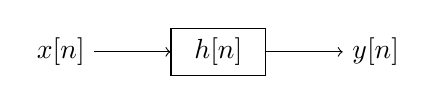
\begin{tikzpicture}
        \node (x) at (0,0) {$x[n]$};
        \node[draw, rectangle, minimum width=1.2cm, minimum height=0.6cm] (h) at (2,0) {$h[n]$};
        \node (y) at (4,0) {$y[n]$};
        \draw[->] (x) -- (h); \draw[->] (h) -- (y);
      \end{tikzpicture}
    \end{center}
    \[
      y[n]=x[n]*h[n]\ \overset{\mathcal{Z}}{\longleftrightarrow}\
      \begin{array}{l}
        Y(z)=X(z)H(z)\\[1mm]
        H(z)=\dfrac{Y(z)}{X(z)}\ :\ \text{Transfer fonksiyonu}\\[3mm]
        h[n]=\mathcal{Z}^{-1}\{H(z)\}\ :\ \text{Dürtü cevabı}
      \end{array}
    \]
\end{enumerate}

\sayfa{8}
\begin{ornek}[]
  $X(z)=\dfrac{az^{-1}}{(1-az^{-1})^2}$, \ $|z|>|a|$, \ $x[n]=\,?$
\end{ornek}
\begin{align*}
  \text{Reminder:}\quad a^nu[n]\ &\overset{\mathcal{Z}}{\longleftrightarrow}\ \frac{1}{1-az^{-1}},\ \ |z|>|a|\\
  n\,a^nu[n]\ &\longleftrightarrow\ -z\frac{d}{dz}\Bigl(\frac{1}{1-az^{-1}}\Bigr)=\frac{az^{-1}}{(1-az^{-1})^2},\ \ |z|>|a|
\end{align*}

\section{ROC ile LTI sistemlerin özelliklerinin analizi}
\begin{enumerate}[label=\arabic*)]
  \item \textbf{Nedensellik:} \ $h[n]=0,\ n<0$ \ sağ yanlı $\longrightarrow$ ROC sağ yanlı\\
    $H(z)$ rasyonel ise paydanın derecesi $>$ payın derecesi olmalıdır\footnote{Claude notu: muhtemelen $\geq$ olmalı; dereceler eşitken de $z\to\infty$ için $H(z)$ sonlu kalır (aşağıdaki örnekte pay ve payda dereceleri eşittir ve $|z|>2$ için sistem nedenseldir).} (aksi durumda $z\to\infty$, $H(z)\to\infty$ gider)
  \item \textbf{Kararlılık:} \ $\displaystyle\sum_{n=-\infty}^{\infty}|h[n]|<\infty\ \longrightarrow$ ROC, birim çemberi içermelidir.
\end{enumerate}

\begin{ornek}[]
  $H(z)=\dfrac{2-\frac52z^{-1}}{\bigl(1-\frac12z^{-1}\bigr)\bigl(1-2z^{-1}\bigr)}$, \ $h[n]=\,?$, \ sistem özellikleri?
\end{ornek}
\[
  H(z)=\frac{2z^2-\frac52z}{z^2-\frac52z+1}=\frac{A}{\bigl(1-\frac12z^{-1}\bigr)}+\frac{B}{\bigl(1-2z^{-1}\bigr)},\qquad A=B=1
\]
$\rightarrow$ $z=0$ ve $z=5/4$ birer sıfır, $z=1/2$ ve $z=2$ birer kutup vardır.
\begin{center}
  \begin{tikzpicture}[scale=1.1]
    \draw[dashed] (0,0) circle (2);
    \draw[murekkep, thick] (0,0) circle (1);
    \draw[->] (-2.4,0) -- (2.8,0) node[right] {Re};
    \draw[->] (0,-2.2) -- (0,2.3) node[above] {Im};
    \draw[thick] (0,0) circle (0.07);
    \node at (0.5,0) {$\times$}; \node at (2,0) {$\times$};
    \draw[thick] (1.25,0) circle (0.07);
    \node[below] at (0.5,-0.1) {\scriptsize$\frac12$};
    \node[above right] at (1,0) {\scriptsize$1$};
    \node[below] at (1.25,-0.1) {\scriptsize$\frac54$};
    \node[below right] at (2,-0.05) {\scriptsize$2$};
  \end{tikzpicture}
\end{center}
1) $|z|>2$
\[
  h[n]=\Bigl(\frac12\Bigr)^nu[n]+2^nu[n]\ \
  \begin{array}{l}
    \longrightarrow h[n]=0,\ n<0 \text{ veya ROC sağ yanlı olduğundan nedensel}\\
    \hookrightarrow \text{ROC, birim çemberi içermediğinden kararlı değil.}
  \end{array}
\]
2) $\frac12<|z|<2$
\[
  h[n]=\Bigl(\frac12\Bigr)^nu[n]-2^nu[-n-1]\ \
  \begin{array}{l}
    \longrightarrow \text{nedensel değil}\\
    \hookrightarrow \text{ROC, birim çemberi içerdiğinden kararlı}
  \end{array}
\]
3) $|z|<1/2$
\[
  h[n]=-\Bigl(\frac12\Bigr)^nu[-n-1]-2^nu[-n-1]\ \
  \begin{array}{l}
    \longrightarrow \text{nedensel değil}\\
    \hookrightarrow \text{kararlı değil}
  \end{array}
\]

\sayfa{9}
\begin{ornek}[]
  $y[n]-\frac12y[n-1]=x[n]+\frac13x[n-1]$ \ ise \ $h[n]=\,?$
\end{ornek}
\[ Y(z)-\frac12z^{-1}Y(z)=X(z)+\frac13z^{-1}X(z) \]
\[
  H(z)=\frac{Y(z)}{X(z)}=\frac{1+\frac13z^{-1}}{1-\frac12z^{-1}}=\frac{z+1/3}{z-1/2}\ \longrightarrow\ z=1/2 \text{ bir kutup vardır.}
\]
$\rightarrow$ $|z|>1/2$
\[ H(z)=\frac{1}{1-\frac12z^{-1}}+\frac13\,\frac{z^{-1}}{1-\frac12z^{-1}} \]
\begin{align*}
  \text{Reminder:}\quad x[n-n_0]\ &\longleftrightarrow\ z^{-n_0}X(z)\\
  a^nu[n]\ &\longleftrightarrow\ \frac{1}{1-az^{-1}},\ \ |z|>|a|
\end{align*}
\[
  h[n]=\Bigl(\frac12\Bigr)^nu[n]+\frac13\Bigl(\frac12\Bigr)^{n-1}u[n-1]\ \longrightarrow\ \text{ROC sağ yanlı ve birim çemberi içerir, nedensel ve kararlı}
\]
$\rightarrow$ $|z|<1/2$
\[
  h[n]=-\Bigl(\frac12\Bigr)^nu[-n-1]-\frac13\Bigl(\frac12\Bigr)^{n-1}u[-n]\ \longrightarrow\ \text{nedensel değil, kararlı değil.}
\]

\medskip
{\color{kirmizikalem}SORU:} \ $x(t)=e^{-2(t-1)}u(t-1)$ 'in FT'nu bulunuz.
\begin{align*}
  \text{\color{yesilkalem}Hatırlatma:}\quad e^{-at}u(t)\ &\longrightarrow\ \frac{1}{a+j2\pi f}\\
  x(t-t_0)\ &\longrightarrow\ e^{-j2\pi ft_0}\cdot X(f)\\
  x(t)=e^{-2(t-1)}u(t-1)\ &\longrightarrow\ e^{-j2\pi f}\,\frac{1}{2+j2\pi f}
\end{align*}

{\color{kirmizikalem}SORU:} \ $x[n]=\bigl(\frac12\bigr)^{n-1}u[n-1]$ 'in FT'nu bulunuz.
\begin{align*}
  \text{\color{yesilkalem}Hatırlatma:}\quad a^nu[n]\ &\longrightarrow\ \frac{1}{1-a\cdot e^{-j\omega}}\\
  x[n-n_0]\ &\longrightarrow\ e^{-j\omega n_0}\cdot X(e^{j\omega})\\
  x[n]=\Bigl(\frac12\Bigr)^{n-1}u[n-1]\ &\longrightarrow\ e^{-j\omega}\,\frac{1}{1-\frac12e^{-j\omega}}
\end{align*}

\sayfa{10}
{\color{kirmizikalem}SORU:} \ $x[n]=\delta[n-1]+\delta[n+1]$
\begin{align*}
  \text{\color{yesilkalem}Hatırlatma:}\quad \delta[n]\ &\longrightarrow\ 1\\
  x[n-n_0]\ &\longrightarrow\ e^{-j\omega n_0}X(e^{j\omega})\\
  x[n]=\delta[n-1]+\delta[n+1]\ &\longrightarrow\ X(e^{j\omega})=e^{-j\omega}+e^{j\omega}=2\cdot\cos(\omega)
\end{align*}

{\color{kirmizikalem}SORU:} \ Fark denklemi: \ $y[n]-\frac12y[n-1]=x[n]-2x[n-1]+x[n-2]$ \ olarak verilen LTI sistemin transfer fonksiyonu $H(e^{j\omega})$'yı bulun.
\begin{align*}
  Y(e^{j\omega})-\tfrac12\cdot e^{-j\omega}\cdot Y(e^{j\omega})&=X(e^{j\omega})-2\cdot e^{-j\omega}X(e^{j\omega})+e^{-j2\omega}X(e^{j\omega})\\
  Y(e^{j\omega})\Bigl[1-\tfrac12e^{-j\omega}\Bigr]&=X(e^{j\omega})\Bigl[1-2\cdot e^{-j\omega}+e^{-j2\omega}\Bigr]
\end{align*}
\[
  \frac{Y(e^{j\omega})}{X(e^{j\omega})}=H(e^{j\omega})=\frac{1-2e^{-j\omega}+e^{-2j\omega}}{1-\frac12e^{-j\omega}}
\]

\begin{enumerate}[label=\arabic*)]
  \item $h[n]=\delta[n]-\delta[n+1]$ ise sistemin birim basamak cevabı nedir?
    \[
      y[n]=h[n]*x[n]=\bigl(\delta[n]-\delta[n+1]\bigr)*u[n]=u[n]*\delta[n]-u[n]*\delta[n+1]=u[n]-u[n+1]=-\delta[n+1]
    \]
  \item $N_0=5$, \ $x[n]=\sin(3\omega_0n)$, \ $k=2$ için FS katsayılarını bulunuz.
    \[ x[n]=\frac{1}{2j}e^{j3\omega_0n}-\frac{1}{2j}e^{-j3\omega_0n} \]
    \[ x_3=\frac{1}{2j}=-j/2\qquad\qquad x_{-3}=-\frac{1}{2j}=j/2 \]
    \[
      x_k=x_{k+N_0}\ \
      \begin{array}{l}
        \longrightarrow x_3=x_8=x_{13}=\cdots\\
        \hookrightarrow x_{-3}=x_2=x_7=\cdots
      \end{array}
    \]
  \item $x(t)=e^{-j2\pi f_0t}$, \ $X(f)=\,?$
    \begin{align*}
      \text{Reminder:}\quad 1\ &\overset{\mathcal{F}}{\longleftrightarrow}\ \delta(f)\\
      e^{\mp j2\pi f_0t}\ &\overset{\mathcal{F}}{\longleftrightarrow}\ \delta(f\pm f_0)
    \end{align*}
    \[ X(f)=\delta(f+f_0) \]
\end{enumerate}

\sayfa{11}
\begin{enumerate}[label=\arabic*), start=4]
  \item $x(t)=2e^{j\pi/2}\sin(2\omega_0t)$, \ $X(f)=\,?$
    \[ x(t)=2j\Bigl[\frac{1}{2j}e^{j2\omega_0t}-\frac{1}{2j}e^{-j2\omega_0t}\Bigr] \]
    \[ \Big\updownarrow\,\mathcal{F} \]
    \[ X(f)=\delta(f-2f_0)-\delta(f+2f_0) \]
  \item $x[n]=e^{j5\pi/2}\sin(3\omega_0n)$, \ $X(e^{j\omega})=\,?$
    \[ x[n]=j\Bigl[\frac{1}{2j}e^{j3\omega_0n}-\frac{1}{2j}e^{-j3\omega_0n}\Bigr] \]
    Reminder: \quad $x[n]=\displaystyle\sum_{k=\langle N\rangle}x_ke^{jk\omega_0n}\ \longleftrightarrow\ X(e^{j\omega})=\sum_{k=-\infty}^{\infty}2\pi x_k\,\delta(\omega-k\omega_0)$
    \[ X(e^{j\omega})=\pi\,\delta(\omega-3\omega_0)-\pi\,\delta(\omega+3\omega_0),\qquad -\pi\leq\omega\leq\pi \]
  \item $N_0=2$, \ $x[n]-x[n-1]$ ifadesinin FS katsayısını bulunuz.
    \[
      \left.
      \begin{array}{l}
        x[n]\ \overset{\text{FS}}{\longleftrightarrow}\ x_k\\[1mm]
        x[n-1]\ \overset{\text{FS}}{\longleftrightarrow}\ e^{-jk\omega_0}x_k
      \end{array}
      \right\}\quad
      \begin{array}{l}
        x[n]-x[n-1]\ \overset{\text{FS}}{\longleftrightarrow}\ (1-e^{-jk\omega_0})x_k=2x_k\\[1mm]
        \omega_0=\dfrac{2\pi}{N_0}=\pi\\[3mm]
        e^{-jk\pi}=\cos(k\pi)-j\sin(k\pi)=-1\text{\footnotemark}
      \end{array}
    \]
    \footnotetext{Claude notu: $\cos(k\pi)=(-1)^k$ olduğundan bu eşitlik yalnızca tek $k$ için geçerlidir; genel olarak katsayı $(1-(-1)^k)x_k$ olur (çift $k$ için $0$, tek $k$ için $2x_k$).}
  \item $x(t)=\frac12\bigl[u(t+1)-u(t-1)\bigr]$\par
    \begin{tikzpicture}[scale=0.7]
      \draw[->] (-1.8,0) -- (2,0) node[right] {$t$};
      \draw[->] (0,-0.2) -- (0,1.6) node[above] {$x(t)$};
      \draw[murekkep, thick] (-1,0) -- (-1,0.9) -- (1,0.9) -- (1,0);
      \node[above right] at (0,0.9) {\scriptsize$1/2$};
      \node[below] at (-1,0) {\scriptsize$-1$}; \node[below] at (1,0) {\scriptsize$1$};
    \end{tikzpicture}\hspace{1cm}
    \begin{minipage}[b]{0.55\linewidth}
      Reminder: \ $A\,\Pi(t/\tau)\ \overset{\mathcal{F}}{\longleftrightarrow}\ A\tau\,\mathrm{sinc}(f\tau)$\par\medskip
      \centering
      \begin{tikzpicture}[scale=0.7]
        \draw[->] (-1.8,0) -- (2,0) node[right] {$t$};
        \draw[->] (0,-0.2) -- (0,1.6);
        \draw[murekkep, thick] (-0.8,0) -- (-0.8,1) -- (0.8,1) -- (0.8,0);
        \node[above right] at (0,1) {\scriptsize$A$};
        \node[below] at (-0.8,0) {\scriptsize$-\tau/2$}; \node[below] at (0.8,0) {\scriptsize$\tau/2$};
      \end{tikzpicture}
    \end{minipage}
    \[ x(t)=\frac12\Pi(t/2)\ \underset{A=1/2,\ \tau=2}{\overset{\mathcal{F}}{\longleftrightarrow}}\ X(f)=\mathrm{sinc}(2f) \]
  \item $x(t)=\mathrm{sinc}(t)$ işaretinin enerjisini ve gücünü bulunuz.
    \[
      \text{Reminder:}\quad
      \left.
      \begin{array}{l}
        x(t)\ \overset{\mathcal{F}}{\longleftrightarrow}\ X(f)\\[1mm]
        X(t)\ \overset{\mathcal{F}}{\longleftrightarrow}\ x(-f)
      \end{array}
      \right\}\ \text{Duality}
    \]
    \begin{minipage}[c]{0.6\linewidth}
      \[ x(t)=\mathrm{sinc}(t)\ \underset{A=\tau=1}{\overset{\mathcal{F}}{\longleftrightarrow}}\ X(f)=\Pi(f) \]
    \end{minipage}\hfill
    \begin{minipage}[c]{0.35\linewidth}
      \centering
      \begin{tikzpicture}[scale=0.7]
        \draw[->] (-1.6,0) -- (1.8,0) node[right] {$f$};
        \draw[->] (0,-0.2) -- (0,1.6) node[above] {$X(f)$};
        \draw[murekkep, thick] (-0.6,0) -- (-0.6,1) -- (0.6,1) -- (0.6,0);
        \node[above right] at (0,1) {\scriptsize$1$};
        \node[below] at (-0.6,0) {\scriptsize$-1/2$}; \node[below] at (0.6,0) {\scriptsize$1/2$};
      \end{tikzpicture}
    \end{minipage}
    Reminder: \quad $E_x=\displaystyle\int_{-\infty}^{\infty}|x(t)|^2\,dt=\int_{-\infty}^{\infty}|X(f)|^2\,df$
    \[
      E_x=\int_{-1/2}^{1/2}1\,df=1<\infty \text{ olduğundan } x(t)=\mathrm{sinc}(t) \text{ enerji işaretidir, } P_x=0\text{'dır.}
    \]
\end{enumerate}

\sayfa{12}
\begin{enumerate}[label=\arabic*), start=9]
  \item $h(t)=e^{2t}u(t)$, \ Kararlılık ve nedensellik?\par
    Reminder: \ $e^{-at}u(t)\ \overset{\mathcal{L}}{\longleftrightarrow}\ \dfrac{1}{s+a},\ \ \mathrm{Re}\{s\}>-a$\par\medskip
    \noindent
    \begin{minipage}[c]{0.3\linewidth}
      $H(s)=\dfrac{1}{s-2},\ \ \mathrm{Re}\{s\}>2$
    \end{minipage}\hfill
    \begin{minipage}[c]{0.25\linewidth}
      \centering
      \begin{tikzpicture}[scale=0.5]
        \begin{scope}
          \clip (2,-1.6) rectangle (3.4,1.8);
          \foreach \i in {-2,-1.5,...,4} \draw[kursunkalem] (\i,-1.6) -- ++(3.4,3.4);
        \end{scope}
        \draw[dashed] (2,-1.6) -- (2,1.8);
        \draw[->] (-1.5,0) -- (3.6,0) node[right] {Re};
        \draw[->] (0,-1.6) -- (0,2) node[above] {Im};
        \node at (2,0) {$\times$};
        \node[below left] at (2,-0.1) {\scriptsize$2$};
      \end{tikzpicture}
    \end{minipage}\hfill
    \begin{minipage}[c]{0.4\linewidth}
      ROC sağ yönlü : Nedensel\\
      ROC $j\omega$ eksenini içermez : Kararlı değil
    \end{minipage}
  \item $1$ ve $-3$'te kutupları olan çift yönlü $x(t)=\,?$\par
    \noindent
    \begin{minipage}[c]{0.66\linewidth}
      \[ X(s)=\frac{1}{(s-1)(s+3)}=\frac{A}{s-1}+\frac{B}{s+3},\qquad A=-B=1/4 \]
      \[ \Big\updownarrow\,\mathcal{L}^{-1} \]
    \end{minipage}\hfill
    \begin{minipage}[c]{0.32\linewidth}
      \centering
      \begin{tikzpicture}[scale=0.5]
        \begin{scope}
          \clip (-3,-1.6) rectangle (1,1.8);
          \foreach \i in {-7,-6.5,...,1} \draw[kursunkalem] (\i,-1.6) -- ++(3.4,3.4);
        \end{scope}
        \draw[dashed] (-3,-1.6) -- (-3,1.8); \draw[dashed] (1,-1.6) -- (1,1.8);
        \draw[->] (-4,0) -- (2.4,0) node[right] {Re};
        \draw[->] (0,-1.6) -- (0,2) node[above] {Im};
        \node at (-3,0) {$\times$}; \node at (1,0) {$\times$};
        \node[below left] at (-3,-0.1) {\scriptsize$-3$};
        \node[below right] at (1,-0.1) {\scriptsize$1$};
        \node[below, align=center, font=\scriptsize] at (-3,-1.7) {$\uparrow$\\sağ yönlü};
        \node[below, align=center, font=\scriptsize] at (1,-1.7) {$\uparrow$\\sol yönlü};
      \end{tikzpicture}
    \end{minipage}
    \[
      x(t)=-Ae^{-t}u(-t)+Be^{-3t}u(t)=\frac{-1}{4}\Bigl(e^{-t}u(-t)+e^{-3t}u(t)\Bigr)\text{\footnotemark}
    \]
    \footnotetext{Claude notu: $s=1$ kutbuna karşılık gelen sol yönlü terim $-Ae^{t}u(-t)$'dir; muhtemelen $e^{-t}$ yerine $e^{t}$ olmalı.}
\end{enumerate}

\end{document}
